% Sección del artículo — dueño: P4.
\section{Resultados}
\subsection{Comparación con las líneas base}
La Tabla~\ref{tab:principal} y la Fig.~\ref{fig:benchmark} resumen
\nfbEpisodiosPorCondicion{} escenarios de prueba por condición. Entre las líneas base, A* con
replanificación resuelve casi todas las misiones con obstáculos fijos
(\nfbExitoAstarNominal{} nominal, \nfbExitoAstarDesconocidos{} con obstáculos no previstos),
pero sólo el \nfbExitoAstarMoviles{} con obstáculos móviles, porque planifica sobre una
fotografía del mapa que queda obsoleta. Sin GPS ninguna supera el
\nfbMejorClasicoSinGPS{}: A* aterriza donde \emph{cree} que está la base, y la deriva de la
odometría lo deja lejos; el retorno ALV corrige parte de ella (\nfbExitoAstarAlvSinGPS{} sin
GPS y \nfbExitoAstarAlvCombinado{} en la condición combinada, frente a \nfbExitoAstarSinGPS{} y
\nfbExitoAstarCombinado{} de A*). Los campos de potencial chocan poco
(\nfbChoquesCampos{}) pero se atascan en mínimos locales.

El híbrido NeuroFly-Bee obtiene \nfbExitoHibridoTotal{} de éxito total
(\nfbExitoHibridoMoviles{} con obstáculos móviles y \nfbExitoHibridoSinGPS{} sin GPS), frente
a \nfbExitoMoscaTotal{} de la mosca sola y \nfbExitoAbejaTotal{} de A* con la red de la abeja.
% P4: comentar aquí, con los números de v19, si el híbrido supera a A*+ALV y dónde no.

\begin{table*}[t]
\centering
\caption{Éxito de misión en la partición de prueba (media $\pm$ d.e. entre semillas de entrenamiento para los controladores neuronales) y tasa total de choques.}
\label{tab:principal}
\begin{tabular}{lcccccccc}
\toprule
Controlador & Nominal & No previstos & Móviles & Viento & Sin GPS & Combinado & Total & Choques \\
\midrule
Directo & 7\% & 0\% & 0\% & 13\% & 0\% & 0\% & 3\% & 95\% \\
Campos de potencial & 77\% & 57\% & 77\% & 80\% & 0\% & 0\% & 48\% & 3\% \\
A* (clásico) & 100\% & 97\% & 40\% & 93\% & 3\% & 0\% & 56\% & 16\% \\
A* + ALV (clásico) & 100\% & 97\% & 40\% & 93\% & 17\% & 23\% & \textbf{62\%} & 16\% \\
A* + supervisor & 100\% & 100\% & 53\% & 93\% & 3\% & 0\% & 58\% & 12\% \\
\bottomrule
\end{tabular}
\end{table*}


\begin{figure*}[t]
\centering
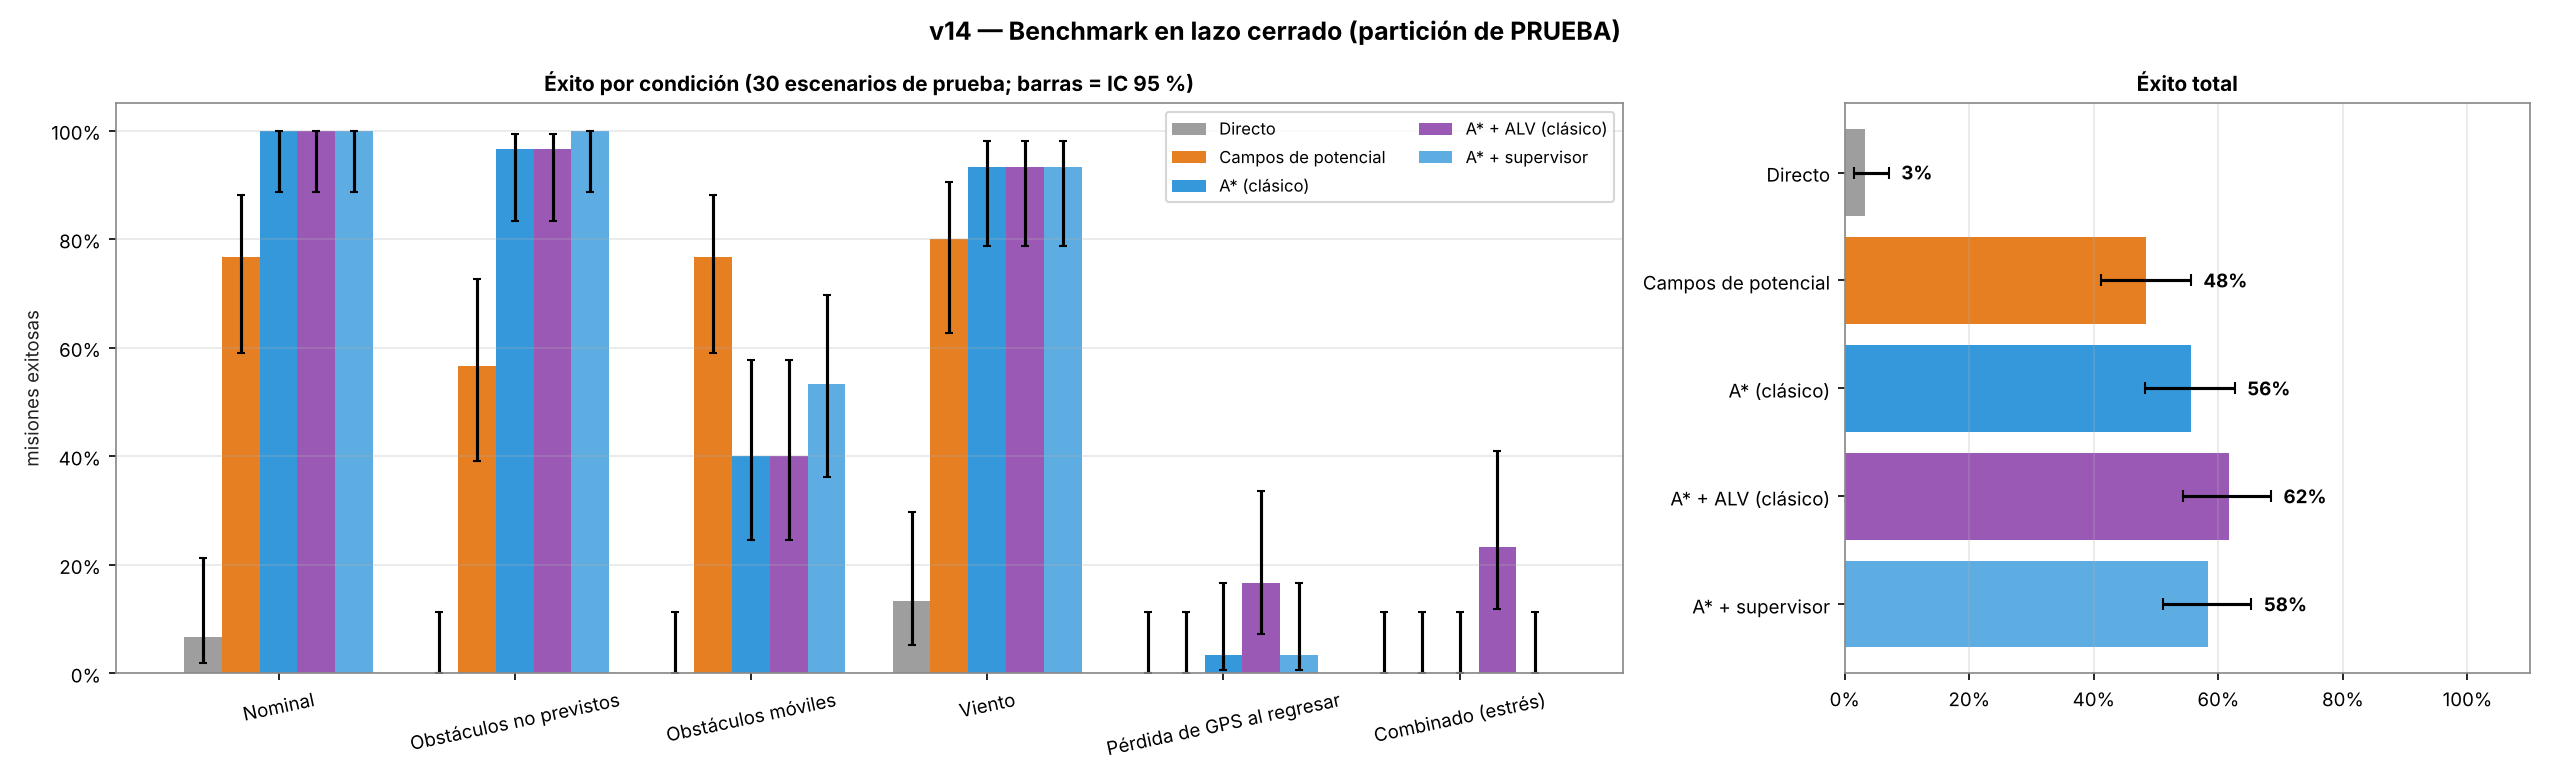
\includegraphics[width=0.9\textwidth]{v14_benchmark}
\caption{Éxito de misión por condición en la partición de prueba (barras de error: IC de
Wilson al 95\,\%).}
\label{fig:benchmark}
\end{figure*}

\subsection{Estudio de ablación}
Cuatro ablaciones aíslan cada decisión de diseño con las mismas semillas de prueba:
(i) arquitectura de la mosca con imitación pura (MLP, CNN, CNN+GRU, CNN+Transformer),
(ii) imitación frente a imitación + DAgger, (iii) retorno sin GPS (ninguno, ALV clásico y red
de la abeja) y (iv) aporte de cada módulo (mosca sola, abeja + mosca, abeja + mosca +
supervisor). En validación, el F1 macro de la mosca es \nfbFUnoMLP{} (MLP), \nfbFUnoCNN{}
(CNN), \nfbFUnoGRU{} (CNN+GRU) y \nfbFUnoTransformer{} (CNN+Transformer), con un AUROC macro
de \nfbAurocGRU{} para CNN+GRU; DAgger lleva el
éxito en lazo cerrado de \nfbDaggerExitoInicial{} a \nfbDaggerExitoFinal{}. La red de la abeja
obtiene en validación un error angular mediano de \nfbAbejaErrorMediano{} frente a
\nfbAlvErrorMediano{} del ALV. Las tablas de ablación del benchmark se regeneran con los pesos
de cada variante.

% Se incluyen las que existan (run_benchmark.py las regenera con los pesos).
\IfFileExists{tablas/v14_ablacion_1.tex}{\input{tablas/v14_ablacion_1}}{}
\IfFileExists{tablas/v14_ablacion_2.tex}{\input{tablas/v14_ablacion_2}}{}
\IfFileExists{tablas/v14_ablacion_3.tex}{\begin{table*}[t]
\centering
\caption{Retorno sin GPS}
\label{tab:ablacion3}
\begin{tabular}{lcccc}
\toprule
Controlador & Sin GPS & Combinado & Total & Choques \\
\midrule
A* sin retorno visual & 3\% & 0\% & 2\% & 17\% \\
A* + ALV clásico & 17\% & 23\% & \textbf{20\%} & 17\% \\
\bottomrule
\end{tabular}
\end{table*}
}{}
\IfFileExists{tablas/v14_ablacion_4.tex}{\input{tablas/v14_ablacion_4}}{}

\subsection{Ablación de la abeja en la partición de prueba}
La Tabla~\ref{tab:ablacion_abeja} y la Fig.~\ref{fig:ablacion_abeja} responden dos preguntas
sobre el diseño siamés, con las mismas semillas, datos e hiperparámetros y sobre
\nfbMuestrasAbejaTest{} vistas de prueba. \emph{¿Hace falta la vista de casa?} Sin ella, la
red obtiene \nfbAblAbejaVistaUnica{} de error mediano, frente a \nfbAblAbejaCompleta{} de la
siamesa; como cada mundo de prueba es distinto, una sola vista sólo puede indicar la base a
través de regularidades del generador de escenarios.
\emph{¿Hace falta la resta explícita?} Sin ella, \nfbAblAbejaSinResta{}.
\emph{¿Hacen falta 172\,547 parámetros?} La lectura vectorial, con
\nfbParamsAbejaCompacta{} parámetros (\nfbAbejaReduccionParams{} veces menos), obtiene
\nfbAblAbejaCompacta{}. El ALV clásico sobre las mismas vistas tiene \nfbAblAbejaAlv{}.
% P4: interpretar aquí con los números de Colab (si la compacta iguala a la plana, el
% argumento de tamaño frente a Bee-Nav queda resuelto).

\begin{table}[t]
\caption{Ablación de la red de la abeja en la partición de prueba (6\,400 vistas; media $\pm$ d.e. entre semillas)}
\label{tab:ablacion_abeja}
\centering
\resizebox{\linewidth}{!}{%
\begin{tabular}{lrrr}
\toprule
Variante & Parámetros & Error mediano (\textdegree) & Error $\le$30\textdegree{} \\
\midrule
ALV clásico & -- & 55.4 & 30\,\% \\
\bottomrule
\end{tabular}}
\end{table}


\begin{figure*}[t]
\centering
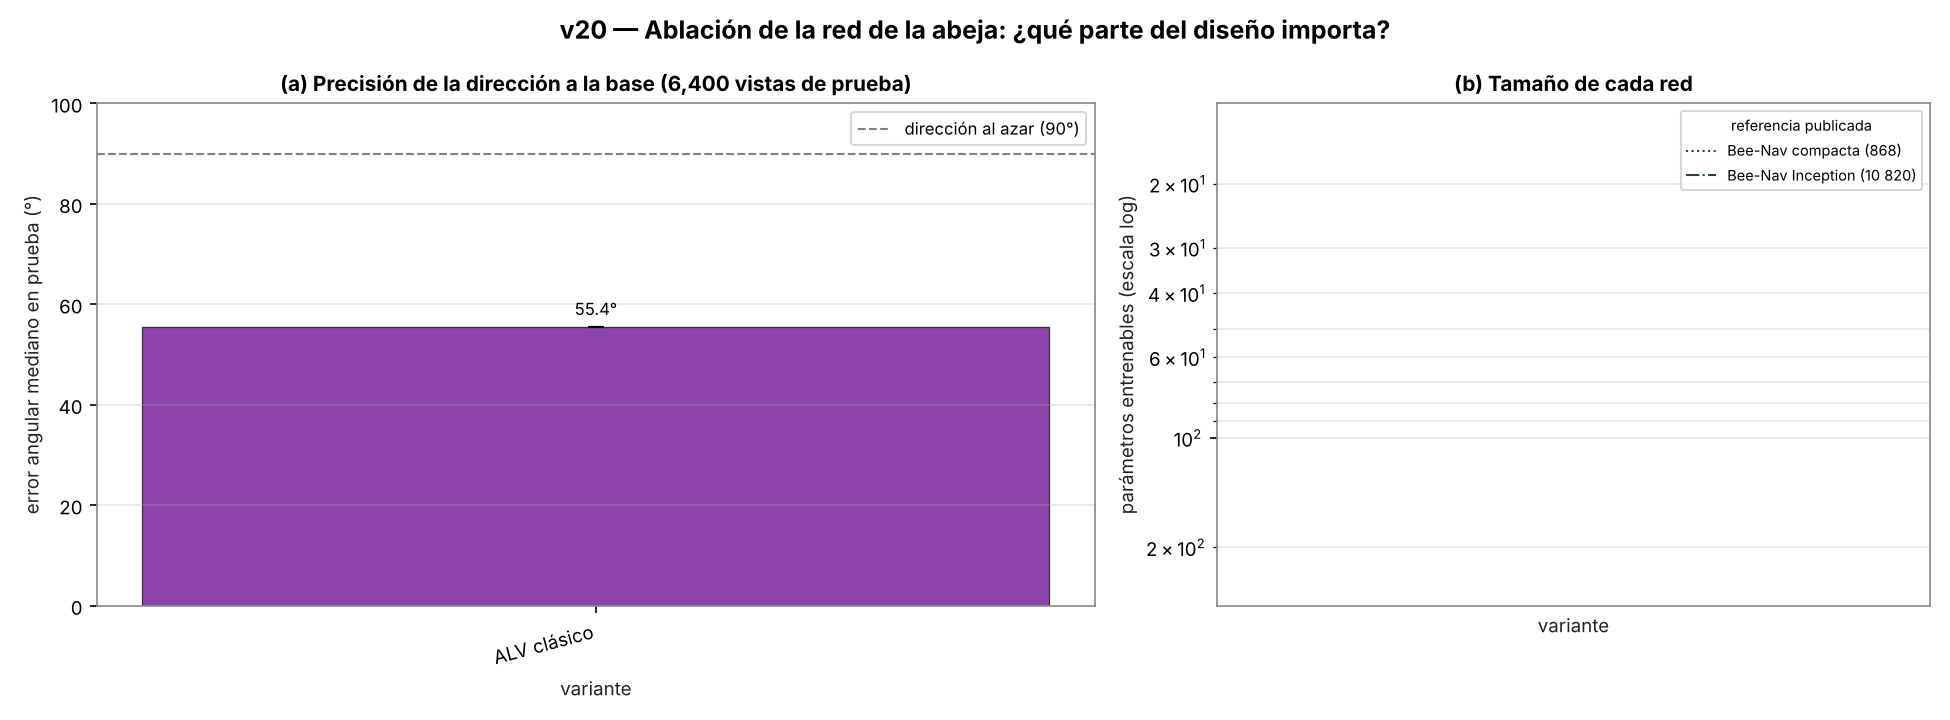
\includegraphics[width=0.95\textwidth]{v20_ablacion_abeja}
\caption{Ablación de la abeja en prueba: (a) error angular mediano (media $\pm$ d.e. entre
semillas; línea punteada: dirección al azar); (b) parámetros en escala logarítmica, con el
tamaño de las redes publicadas de Bee-Nav~\cite{ou2026} como referencia.}
\label{fig:ablacion_abeja}
\end{figure*}

\subsection{Significancia estadística}
La Tabla~\ref{tab:significancia} reúne las comparaciones pareadas;
\nfbSigSignificativas{} de \nfbSigComparaciones{} son significativas tras la corrección de
Holm. Entre las líneas base, el retorno ALV mejora a A* en \nfbSigAlvAstarTotalDif{} de
éxito total (\nfbSigAlvAstarTotalP{}). El híbrido frente a A*+ALV difiere en
\nfbSigHibridoAlvTotalDif{} en total (\nfbSigHibridoAlvTotalP{}) y en
\nfbSigHibridoAlvSinGPSDif{} sin GPS (\nfbSigHibridoAlvSinGPSP{}). Con 30 escenarios por
condición y una corrección conservadora, diferencias de unos 10 puntos pueden no alcanzar
significancia; por eso se reportan siempre el intervalo y el tamaño de efecto.

\begin{table*}[t]
\caption{Comparaciones pareadas sobre los mismos escenarios de prueba: diferencia de éxito $\Delta$ con IC 95\,\% bootstrap, valor $p$ de la permutación pareada corregido por Holm y $h$ de Cohen. En negrita, $p_{\text{Holm}}<0.05$.}
\label{tab:significancia}
\centering
\resizebox{\textwidth}{!}{%
\begin{tabular}{llllrrrrrr}
\toprule
Grupo & A & B & Condición & $n$ & Éxito A & Éxito B & $\Delta$ [IC 95\,\%] & $p_{\text{Holm}}$ & $h$ \\
\midrule
Principal & A$^*$ + ALV (clásico) & A$^*$ (clásico) & todas & 180 & 62\,\% & 56\,\% & +6 [+3, +10] & \textbf{0.017} & +0.12 \\
Principal & A$^*$ + ALV (clásico) & A$^*$ (clásico) & sin GPS & 30 & 17\,\% & 3\,\% & +13 [+0, +30] & 0.539 & +0.47 \\
Principal & A$^*$ + ALV (clásico) & A$^*$ (clásico) & combinada & 30 & 23\,\% & 0\,\% & +23 [+10, +40] & 0.062 & +1.01 \\
Principal & A$^*$ + supervisor & A$^*$ (clásico) & todas & 180 & 58\,\% & 56\,\% & +3 [-1, +6] & 0.539 & +0.06 \\
Principal & A$^*$ + supervisor & A$^*$ (clásico) & móviles & 30 & 53\,\% & 40\,\% & +13 [-3, +30] & 0.539 & +0.27 \\
\bottomrule
\end{tabular}}
\end{table*}

